% Author: Hadrian Lau
% Website: https://www.hadrian.cc
% License: LaTeX Project Public License (LPPL)

\documentclass[a4paper,12pt]{article}

% Packages
\usepackage[utf8]{inputenc}
\usepackage[english]{babel}
\usepackage{amsmath, amsthm, amssymb, amsfonts}
\usepackage{graphicx}
\usepackage{setspace}
\usepackage{geometry}
\usepackage{float}
\usepackage{framed}
\usepackage[dvipsnames,svgnames]{xcolor}
\usepackage[most]{tcolorbox}
\usepackage{thmtools}
\usepackage{apacite}
\usepackage{indentfirst}
\usepackage{parskip}
\usepackage{chemfig}
\usepackage{pgfplots}
\usepackage[version=4,arrows=pgf-filled,mathfontname=mathsf]{mhchem}
\usepackage{fancyhdr}
\usepackage{titlesec}
\usepackage{xpatch}
\usepackage{blindtext}
\usepackage{hyperref}
\usepackage{empheq}

% Settings
\pgfplotsset{width=15cm,compat=1.18}
\geometry{margin=1in}
\setstretch{1.5}
\newcommand{\HRule}[1]{\rule{\linewidth}{#1}}

% Box equations
\makeatletter
\newcommand{\colorboxed}[1]{\fcolorbox{DarkSeaGreen}{DarkSeaGreen!20}{\m@th$\displaystyle#1$}}
\xpatchcmd{\@Aboxed}{\boxed}{\colorboxed}{}{}
\makeatother

% Note sections
\makeatletter
\NewDocumentCommand{\mynote}{+O{}+m}{%
	\begingroup
	\tcbset{%
		noteshift/.store in=\mynote@shift,
		noteshift=1.5cm
	}
	\begin{tcolorbox}[nobeforeafter,
		enhanced,
		sharp corners,
		toprule=1pt,
		bottomrule=1pt,
		leftrule=0pt,
		rightrule=0pt,
		colback=DarkSeaGreen!20,
		#1,
		left skip=\mynote@shift,
		right skip=\mynote@shift,
		overlay={\node[right] (mynotenode) at ([xshift=-\mynote@shift]frame.west) {\textbf{Note:}} ;},
		]
		#2
	\end{tcolorbox}
	\endgroup
}
\makeatother

% Header and Footer
\pagestyle{fancy}
\fancyhf{}
\fancyhead[L]{Pendulum and Projectile Motion} % HERE
\fancyhead[R]{\thepage}

% Document
\begin{document}
	
	% Front page
	\title{ \normalsize \textsc{}
		\\ [2.0cm]
		\HRule{1.5pt} \\
		\LARGE \textbf{
			\uppercase{Pendulum and Projectile Motion} % HERE
			\HRule{2.0pt} \\ [0.6cm] 
			\LARGE{SPH3U Unit 1 Lab} % HERE
			\vfill
		}
	}
	\date{}
	\author{
		\textbf{Hadrian Lau Yiu Hei} \\ 
		\textbf{Ms. Rashmi Shroff}\\
		Sin Chi Lam, Jae-Hee Han, Sadan Ahmed Shaikh, Brinstan Lo, Junho Song \\
		26th September, 2025\\ %HERE
		\href{https://hadrian.cc}{{\color{blue}\underline{\LaTeX\, document code}}}
	}
	\maketitle
	\thispagestyle{empty}
	
	\newpage

	% Table of content
	\setcounter{page}{1}
	\tableofcontents
	\newpage
	
	% Content
	\section{Pendulum Motion}
	The purpose of the pendulum motion lab is to determine the acceleration due to gravity. A pendulum with a string length of 0.33m, attached with a 1.5cm in diameter steel ball, is dropped from a $5^\circ$ from the right without external forces. We recorded the time it takes for 10 oscillations for a total of 3 times for maximum accuracy. 
	
	\subsection{Raw data}
	Length of pendulum wire: $L=33\text{cm}=0.33\text{m}$\\
	Initial angular displacement: $\theta=5^\circ$ to the right\\
	
	\subsubsection{Trials}
	We did a total of 3 trials, each measuring the time for 10 pendulum oscillations to occur:
	\begin{align*}
		t_1&=11.66\text{s}\\
		t_2&=11.85\text{s}\\
		t_3&=11.65\text{s}
	\end{align*}\\
	\subsection{Trial calculations}
	The average actual time for 10 oscillations is:
	\begin{align*}
		t_{10avg}&=\frac{11.66\text{s}+11.85\text{s}+11.65\text{s}}{3}\\
		&=\frac{35.16\text{s}}{3} \\
		t_{10avg}&=11.72\text{s}\\
	\end{align*}
	
	So, the average actual time for 1 oscillations is:
	\begin{align*}
		t_{avg}&=\frac{11.72\text{s}}{10}\\
		\Aboxed{t_{avg}&=1.17\text{s}}
	\end{align*}
	
	\subsection{Theoretical time}
	We can calculate the theoretical time for each oscillation under perfect conditions using the simple harmonic motion equation:
	\begin{align*}
		t_{the}&=2\pi\times\sqrt{\frac{L}{g}}\\
		&=2\pi\times\sqrt{\frac{0.33\text{m}}{9.81\text{m}/\text{s}^2}}  \\
		&=2\pi\times\sqrt{0.034\text{s}^2}\\
		&=2\pi\times 0.183\text{s} \\
		\Aboxed{t_{the}&=1.15\text{s}}
	\end{align*} 
	
	\subsection{Error sources}
	Our actual time measurements are quite accurate. There is a very small difference between our actual time and the theoretical time:
	\begin{align*}
		\Delta&=1.17\text{s}-1.15\text{s} \\
		&=0.02\text{s}\\
	\end{align*}
	
	This marginal time difference of 20 milliseconds can be caused by errors like:
	\begin{itemize}
		\item Human error
		\item Theoretical value of g is not the same around the world
		\item Air resistance
	\end{itemize}
	\subsection{Experiment optimization}
	
	\newpage
	
	\section{Projectile motion}
	The purpose of the projectile motion lab is to determine the properties of a projectile through displacement graphs, velocity graphs, and a variety of data. We placed a steel ball at the top of the ramp, and captured the trajectory of the steel ball using a slow motion camera.
	
	\subsection{Raw data}
	Each grid's length: 2cm=0.2m\\
	Each grid's width: 2cm-0.2m\\
	Steel ball diameter: 1.5cm = 0.015m
	
	After reviewing the slow motion video, we can compile the following data points:
	\begin{center}
		\begin{tabular}{ |c|c|c| } 
			\hline
			$\vec{\Delta d_x}$ (m [$\rightarrow$]) & $\vec{\Delta d_y}$ (m [$\uparrow$]) & t (s)\\ 
			\hline\hline
			0.00m & 0.20m & 0.00s\\
			\hline 
			0.02m & 0.19m & 0.03s\\ 
			\hline
			y0.04m & 0.17m & 0.06s\\
			\hline
			0.06m & 0.14m & 0.09s \\
			\hline
			0.08m & 0.10m & 0.12s\\
			\hline
			0.10m & 0.05m & 0.15s \\
			\hline
			0.12m & 0.00m & 0.18s\\
			\hline
		\end{tabular} 
	\end{center}
	\bigskip
	\mynote{We measured everything using the steel ball's bottom.}
	\mynote{The steel ball is tracked using a 2cm grid plane. These values are obtained by scaling the values obtained on the grid plane.}
	
	\newpage
	
	\subsection{Calculations}
	All calculations are based on the table of values. 
	\subsubsection{Total Displacement (x-axis)}
	The total displacement in the x-axis:
	\begin{align*}
		\vec{\Delta d}_x&=\vec{\Delta d}_{xf}-\vec{\Delta d}_{xi}\\
		&=0.12 \text{m}\;[\rightarrow]-0.0 \text{m}\; [\rightarrow]\\
		\Aboxed{\vec{\Delta d}_x&=0.12\text{m}\; [\rightarrow]}
	\end{align*}
	\subsubsection{Total Displacement (y-axis)}
	The total displacement in the y-axis
	\begin{align*}
		\vec{\Delta d}_y&=\vec{\Delta d}_{yf}-\vec{\Delta d}_{yi}\\
		&=0.00 \text{m}\; [\uparrow]-0.20 \text{m}\; [\uparrow]\\
		&=-0.20\text{m}\; [\uparrow]\\
		\Aboxed{\vec{\Delta d}_y&=0.20\text{m}\; [\downarrow]}
	\end{align*}
	\subsubsection{Initial Velocity \& Final Velocity (x-axis)}
	According to the laws of projectile motion, $\vec{v_{ix}}=\vec{v_{fx}}$.
	\begin{align*}
		\vec{\Delta d}_x&=\frac{\vec{v_{ix}}+\vec{v_{fx}}}{2}\times \Delta t\\
		&=\frac{2\vec{v_x}}{2}\times \Delta t\\
		&=\vec{v_x}\times \Delta t\\
		0.12\text{m}\; [\rightarrow]&=\vec{v_x} \times 0.18\text{s}\\
		\vec{v_x}&=\frac{0.12\text{m}\; [\rightarrow]}{0.18\text{s}}\\
		\vec{v_x}&=0.67\text{m}/\text{s}\;[\rightarrow]\\
		\Aboxed{\vec{v_{ix}}=\vec{v_{fx}}&=0.67\text{m}/\text{s}\;[\rightarrow]}
	\end{align*}
	\subsubsection{Initial Velocity (y-axis)}
	Since we did not push the steel ball downwards, gravity is the only force that affects it. Hence, when the steel ball is slid down from the ramp, then:
	\begin{align*}
		\Aboxed{\vec{v_{iy}}&=0\text{m}/\text{s}\;[\emptyset]}\\
	\end{align*}
	\subsubsection{Final Velocity (y-axis)}
	The final velocity in the y-axis:
	\begin{align*}
		\vec{\Delta d}_y&=\Delta t\left(\vec{v}_{fy}-\frac{1}{2}\vec{a}_y\Delta t\right)\\
		0.20\text{m}\;[\downarrow]&=0.18\text{s}\left(\vec{v}_{fy}-\frac{1}{2}\left(9.81\text{m}/\text{s}^2\;[\downarrow]\right)0.18\text{s}\right)\\
		\frac{0.20\text{m}\;[\downarrow]}{0.18\text{s}}&=\vec{v}_{fy}-\frac{1}{2}\times9.81\text{m}/\text{s}^2\;[\downarrow]\times0.18\text{s}\\
		1.1\text{m}/\text{s}\;[\downarrow]&=\vec{v}_{fy}-0.83\text{m}/\text{s}\;[\downarrow]\\
		\Aboxed{\vec{v}_{fy}&=1.93\text{m}/\text{s}\;[\downarrow]}
	\end{align*}
	\newpage
	\subsection{Position-Time graph}
	Using the table of values, where the displacement on the y-axis ($\vec{\Delta d}_y$) in $\text{m} \,[\rightarrow]$ (meters) is the y-axis and the time (t) in s (seconds), we can plot a graph using the following table:
	\begin{center}
		\begin{tabular}{ |c|c| } 
			\hline
			$\vec{\Delta d_y}$ (m [$\uparrow$]) & t (s)\\ 
			\hline\hline
			0.20m & 0.00s\\
			\hline 
			0.19m & 0.03s\\ 
			\hline
			0.17m & 0.06s\\
			\hline
			0.14m & 0.09s \\
			\hline
			0.10m & 0.12s\\
			\hline
			0.05m & 0.15s \\
			\hline
			0.00m & 0.18s\\
			\hline
		\end{tabular} 
	\end{center}
	
	\subsubsection{Theoretical displacement equation}
	We included the theoretical graph as a comparison for error sources:
	\begin{align*}
		\vec{\Delta d}_y&=\Delta t\left(\vec{v}_{iy}+\frac{1}{2}\vec{a}_y\Delta t\right)\\
		\vec{\Delta d}_y&=\Delta t\left(0+\frac{1}{2}(-9.81 \text{m}/\text{s}^2\;[\uparrow])\Delta t\right)\\
		\vec{\Delta d}_y&=-4.905 \text{m}/\text{s}^2\;[\uparrow]\times\Delta t^2\\
	\end{align*}
	Since we are dropping from a height of 0.158m, we get the following equation:
	\begin{align*}
		\vec{\Delta d}_y&=0.20-4.905 \text{m}/\text{s}^2\;[\uparrow]\times\Delta t^2\\
		\Aboxed{\vec{\Delta d}_y&=0.2-4.905t^2}
	\end{align*}
	
	\subsubsection{Position-Time graph}
	\begin{center}
		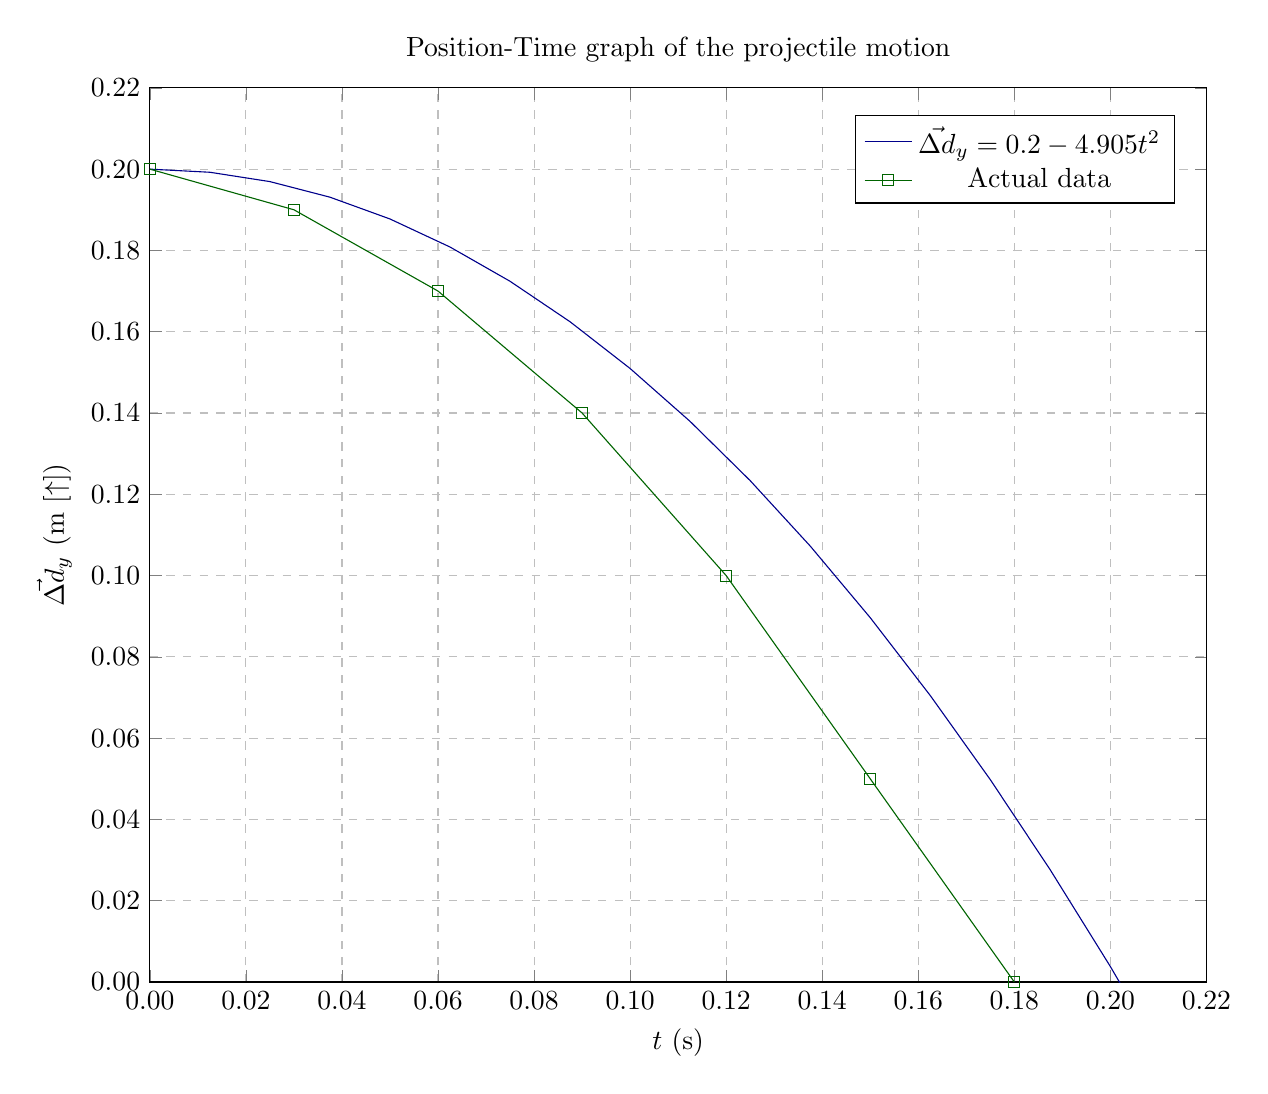
\begin{tikzpicture}
			\begin{axis} [
				title={Position-Time graph of the projectile motion},
				xlabel={$t$ (\text{s})},
				ylabel={$\vec{\Delta d}_y$ (\text{m} [$\uparrow$])},
				xmin=0, xmax=0.22,
				ymin=0, ymax=0.22,
				y tick label style={/pgf/number format/fixed,
					/pgf/number format/fixed zerofill={true}},
				x tick label style={/pgf/number format/fixed,
					/pgf/number format/fixed zerofill={true}},
				xtick distance=0.02,
				ytick distance=0.02,
				ymajorgrids=true,
				xmajorgrids=true,
				legend pos=north east,
				grid style=dashed,
				]	
				\addplot[
				color=DarkBlue,
				domain=0:0.3,
				] {
					0.2-4.905*x*x
				};
				\legend{$\vec{\Delta d}_y=0.2-4.905t^2$, Actual data}
				\addplot[
				color=DarkGreen,
				mark=square,
				] coordinates {
					(0,0.2)(0.03,0.19)(0.06,0.17)(0.09,0.14)(0.12,0.10)(0.15,0.05)(0.18,0)
				};
			\end{axis}
		\end{tikzpicture}
	\end{center}
	\newpage
	\subsection{Velocity-Time graph}
	There are no raw data for the veocity of the steel ball. Hence, we need to calculate the equation of the velocity by taking the derivative of the equation

	By entering the data points in Google Sheets, we get the following equation for the curve of best fit of the position time graph:
	\begin{align*}
	V(t)=-4.89t^2-0.25t+0.201 
	\end{align*}
	
	Take the derivative of $V(t)$:
	\begin{align*}
		V(t)&=-4.89t^2-0.25t+0.201 \\
		V'(t)&=-4.89(2t)-0.25+0\\
		\Aboxed{V'(t)&=-9.78t-0.25}
	\end{align*}
	\subsubsection{Theoretical velocity equation}
	We included the theoretical graph as a comparison for error sources:
	\begin{align*}
		\vec{a}_y&=\frac{\vec{v}_{fy}-\vec{v}_{iy}}{\Delta t}\\
		-9.81\text{m}/\text{s}^2\;[\uparrow]&=\frac{\vec{v}_{fy}-0}{\Delta t}\\
		-9.81\text{m}/\text{s}^2\;[\uparrow]\times\Delta t&=\vec{v}_{fy}\\
		\Aboxed{\vec{v}_y&=-9.81t}
	\end{align*}
	
	\subsubsection{Velocity-Time graph}
	\begin{center}
		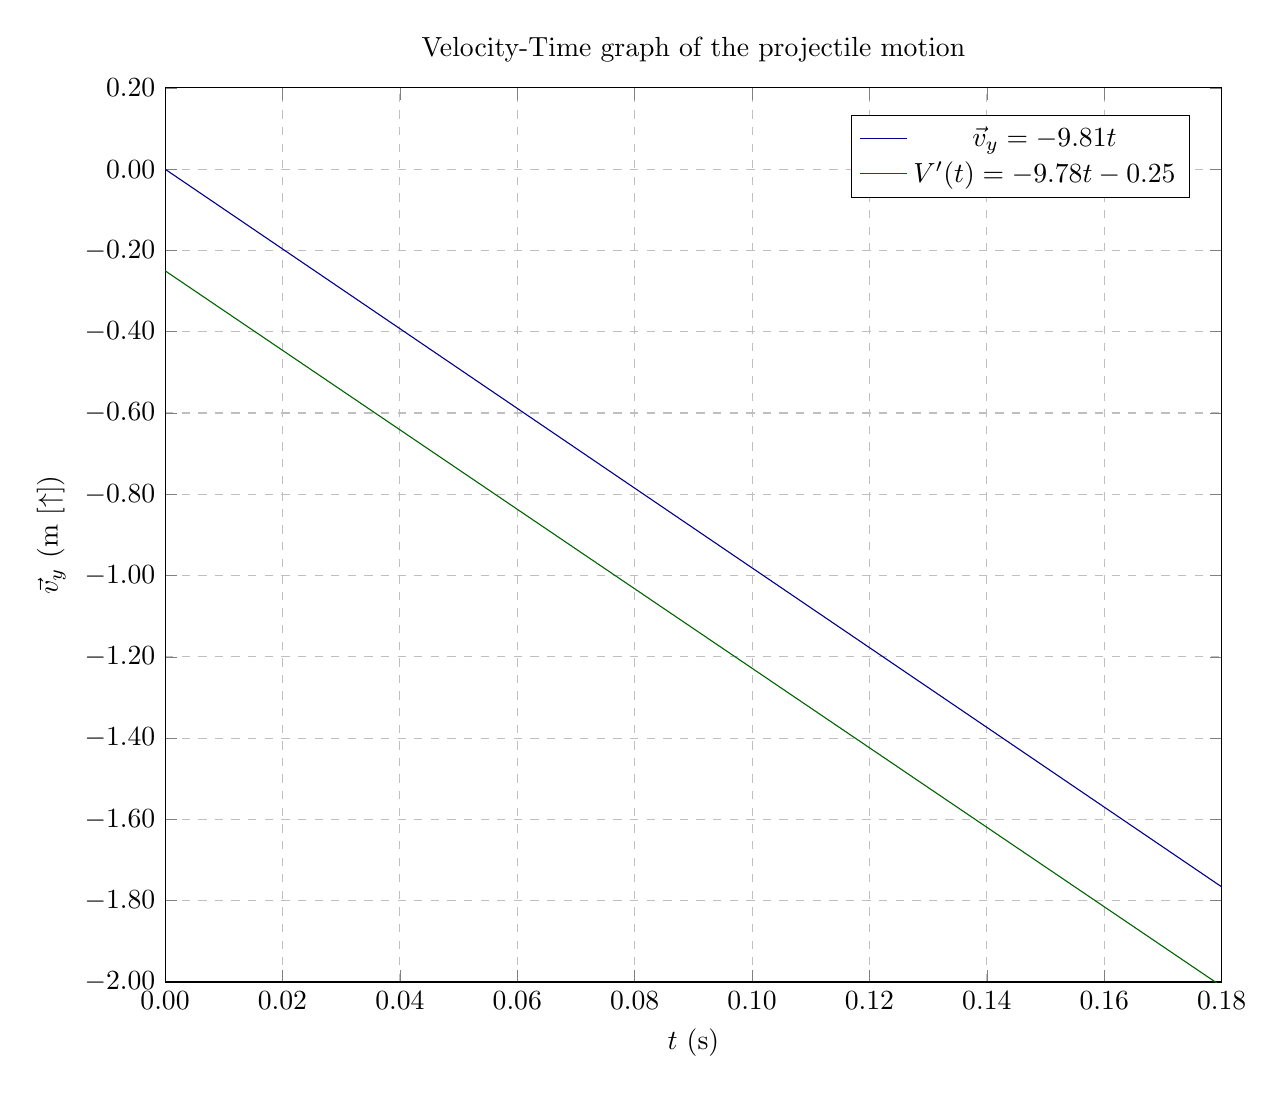
\begin{tikzpicture}
			\begin{axis} [
				title={Velocity-Time graph of the projectile motion},
				xlabel={$t$ (\text{s})},
				ylabel={$\vec{v}_y$ (\text{m} [$\uparrow$])},
				xmin=0, xmax=0.18,
				ymin=-2, ymax=0.2,
				y tick label style={/pgf/number format/fixed,
					/pgf/number format/fixed zerofill={true}},
				x tick label style={/pgf/number format/fixed,
					/pgf/number format/fixed zerofill={true}},
				xtick distance=0.02,
				ytick distance=0.2,
				ymajorgrids=true,
				xmajorgrids=true,
				grid style=dashed,
				legend pos=north east,
				]			
				\addplot[
					color=DarkBlue,
					domain=0:0.18,
				] {
					-9.81*x
				};
				\legend{$\vec{v}_y=-9.81t$, $V'(t)=-9.78t-0.25$}
				\addplot[
					color=DarkGreen,
					domain=0:0.18,
				] {
					-9.78*x-0.25
				};
			\end{axis}
		\end{tikzpicture}
	\end{center}
	
	\subsection{Error sources}
	The position-time graph has similar curves as the theoretical graph, but the values differ as the time increases.
	
	The velocity-time graph is linear like the theoretical graph, but the values differ because of errors from the position-time graph. 
	
	\subsection{Experiment optimization}
	
	\newpage
	\section{Licensing}
	\subsection{Packages}
	All \LaTeX\, packages are provided by TeX Live under the LaTeX Project Public License (LPPL).\\
	
	\subsection{Tools}
	The \LaTeX\, engine is provided by TeX Live under the LaTeX Project Public License (LPPL).\\
	
	The \LaTeX\, code editor is provided by TeXstudio under the GNU General Public License (GPL) version 2.\\
	
	The \LaTeX\, typesetting system is distributed under the LaTeX Project Public License (LPPL).\\
	
	The NixOS Linux Operating System is distributed under the GNU Lesser General Public License (LGPL) version 2.1.\\
	
	%\newpage
	%\bibliographystyle{plain}
	%\bibliography{references}  % Add a .bib file if you have references
	
\end{document}

% All LaTeX packages are provided by TeX Live under the LaTeX Project Public License (LPPL).
% The pgfplots package is licensed under the GNU General Public License (GPL) version 3 or later.
% The titlesec package is licensed under the MIT License.
% The LaTeX engine is provided by TeX Live under the LaTeX Project Public License (LPPL).
% NixOS Linux Operating System is distributed under the GNU Lesser General Public License (LGPL) version 2.1.
% The LaTeX code editor is provided by TeXstudio under the GNU General Public License (GPL) version 2.
% The LaTeX typesetting system is distributed under the LaTeX Project Public License (LPPL).


